\section{Les environnements flottants}
\subsection{Les figures}

\begin{frame}[fragile]
  \frametitle{Figures I}
  \begin{itemize}

  \item Utilisation du package \lstinline|\usepackage{graphicx}|
  \item Insertion de l'image avec \lstinline|\includegraphics[options]{filename.ext}|

  \item \textbf{Non-flottant}

    Référencement par ``ci-dessous'', \dots
    \begin{lstlisting}[style=nonumbers]
\begin{center}
  \includegraphics{image.jpg}
\end{center}
    \end{lstlisting}

  \item \textbf{Flottant}
      \begin{itemize}
          \item Environnement \lstinline|figure|
          \item Ajout d'une référence par \lstinline|\label{...}|
        \item Référencement par \lstinline|voir figure \ref{fig:graphique}|
        \item Ajout d'une légende par \lstinline|\caption{...}|
    \end{itemize}
    \begin{lstlisting}[style=nonumbers]
\begin{figure}
  \centering
  \includegraphics{graph.png}
  \caption{Voici un beau graphique}
  \label{fig:graphique}
\end{figure}
    \end{lstlisting}
\end{itemize}
\end{frame}

\begin{frame}[fragile]
  \frametitle{Référencer des éléments du texte}
  Pour faire référence à une page, section, figure, table, équation mathématique, \dots:
  \begin{itemize}
    \item Mettre une étiquette (label) à l'endroit à référencer
      \begin{itemize}
        \item \lstinline|\label{identifiant}|.
      \end{itemize}
    \item Mettre une référence à cette étiquette :
      \begin{itemize}
        \item \lstinline|\ref{identifiant}| pour le numéro de section, figure, table, équation;
        \item \lstinline|\pageref{identifiant}| pour le numéro de page;
      \end{itemize}
  \end{itemize}
  \begin{columns}
    \begin{column}{0.5\textwidth}
      \begin{lstlisting}[style=nonumbers]
  \label{ref}
  Nous sommes section \ref{ref},
  page \pageref{ref},
      \end{lstlisting}
    \end{column}
    \begin{column}{0.5\textwidth}
      \label{ref:id}
      \par{}Nous sommes section~\ref{ref:id},
      page~\pageref{ref:id},
    \end{column}
  \end{columns}
\end{frame}

\begin{frame}[fragile]\
  \frametitle{Figures II}
  \begin{itemize}

    \item \textbf{Scaling}
  \begin{lstlisting}[style=nonumbers]
\includegraphics[width=0.7\textwidth]{image.jpg} % Largeur dépendant du texte
\includegraphics[height=4cm]{image.jpg} % Hauteur de 4cm
\includegraphics[scale=0.5]{image.png} % taille de l'image / 2
  \end{lstlisting}

  \vspace{2em}
  \end{itemize}
\end{frame}

\begin{frame}[fragile]{Exemple de figure}
  \begin{columns}
    \begin{column}{0.5\textwidth}
    \begin{lstlisting}[style=nonumbers]

    Sur la figure \ref{fig:uclLogo}, vous pouvez
    voir le logo UCLouvain mis a 50\%
    de la largeur du texte.

    \begin{figure}
        \centering
        
\includegraphics[width=0.50\textwidth]{logo-uclouvain.eps}
        \caption{Voici le logo UCLouvain}
        \label{fig:uclLogo}
    \end{figure}
    \end{lstlisting}
    \end{column}
    \begin{column}{0.5\textwidth}
    Sur la figure \ref{fig:uclLogo}, vous pouvez voir le logo UCLouvain
    mis a \SI{50}{\percent} de la largeur du texte.

    \begin{figure}[!ht]
        \centering
        
\includegraphics[width=0.50\textwidth]{logo-uclouvain.pdf}
        \caption{Voici le logo UCLouvain}
        \label{fig:uclLogo}
    \end{figure}
    \end{column}
  \end{columns}
\end{frame}

\subsection{Les tableaux}

\begin{frame}[fragile,allowframebreaks]
  \frametitle{Tableaux}
  \begin{itemize}
    \item \textbf{Code}
      \begin{lstlisting}[style=nonumbers]
\begin{tabular}{<colonnes>}
  <lignes>
\end{tabular}
      \end{lstlisting}
      \begin{itemize}
          \item Définition de l'alignement des <colonnes> par :
              \begin{itemize}
                  \item un \lstinline|l| pour aligner à gauche (\textit{left})
                  \item un \lstinline|c| pour centrer (\textit{center})
                  \item un \lstinline|r| pour aligner à droite (\textit{right})
                  \item un \lstinline|p{<largeur>}| pour un texte justifié sur une largeur donnée
              \end{itemize}
          \item Une ligne verticale est tracée par \lstinline|||
          \item Le contenu des <lignes> est séparé par colonne grâce à des \lstinline|&|
          \item Une <ligne> se termine par \lstinline|\\|
          \item Une ligne horizontale est tracée par \lstinline|\hline|
      \end{itemize}\framebreak
    \item \textbf{Exemple}
    \begin{lstlisting}
\begin{tabular}{|lcrp{0.25\textwidth}|}
  \hline
  Gauche & Centré & Droite & Justifié\\
  \hline
  a & b & c & Le texte est trop long.\\
  1 & 2 & 3 & Il passe donc à la ligne suivante.\\
  \hline
\end{tabular}
        \end{lstlisting}
      \item \textbf{Rendu}
    \begin{table}[!ht]
    \centering
    \begin{tabular}{|lcrp{0.25\textwidth}|}
      \hline
      Gauche & Centré & Droite & Justifié\\
      \hline
      a & b & c & Le texte est trop long.\\
      1 & 2 & 3 & Il passe donc à la ligne suivante.\\
      \hline
    \end{tabular}
    \end{table}
    \framebreak

      \item \textbf{Non-flottant}

    Référencement par ''ci-dessous'', \dots
    \begin{lstlisting}[style=nonumbers]
\begin{center}
    \begin{tabular}{...}
        ...
    \end{tabular}
\end{center}
    \end{lstlisting}

  \item \textbf{Flottant}
      \begin{itemize}
          \item Environnement \lstinline|table|
        \item Référencement par \lstinline|voir tableau \ref{tab:data}|
    \end{itemize}
    \begin{lstlisting}
\begin{table}
  \centering
  \begin{tabular}{...}
    ...
  \end{tabular}
  \caption{Voici un beau tableau}
  \label{tab:data}
\end{table}
    \end{lstlisting}
  \end{itemize}
\end{frame}

\begin{frame}[fragile]{Exemple de tableau}
  \begin{footnotesize}
  \begin{lstlisting}[style=nonumbers]
  \begin{table}
    \begin{center}
      \begin {tabular}{|l||c|} %% 2 columns
        \hline
        \textit{Inventaire} & \textbf{Nombre} \\
        \hline
        Chemises  & 4   \\
        Pulls     & 12  \\
        Pantalons & 1   \\
        \hline
      \end{tabular}
      \caption{Tableau relatif a l'inventaire}
    \end{center}
  \end{table}
  \end{lstlisting}
  \end{footnotesize}
  \begin{center}
  \fbox{\includegraphics[width=0.6\textwidth]{table.jpg}}
  \end{center}
\end{frame}

\subsection{Exercice 2}

\begin{frame}[fragile]{Deuxième exercice}
  \begin{center}
      \fbox{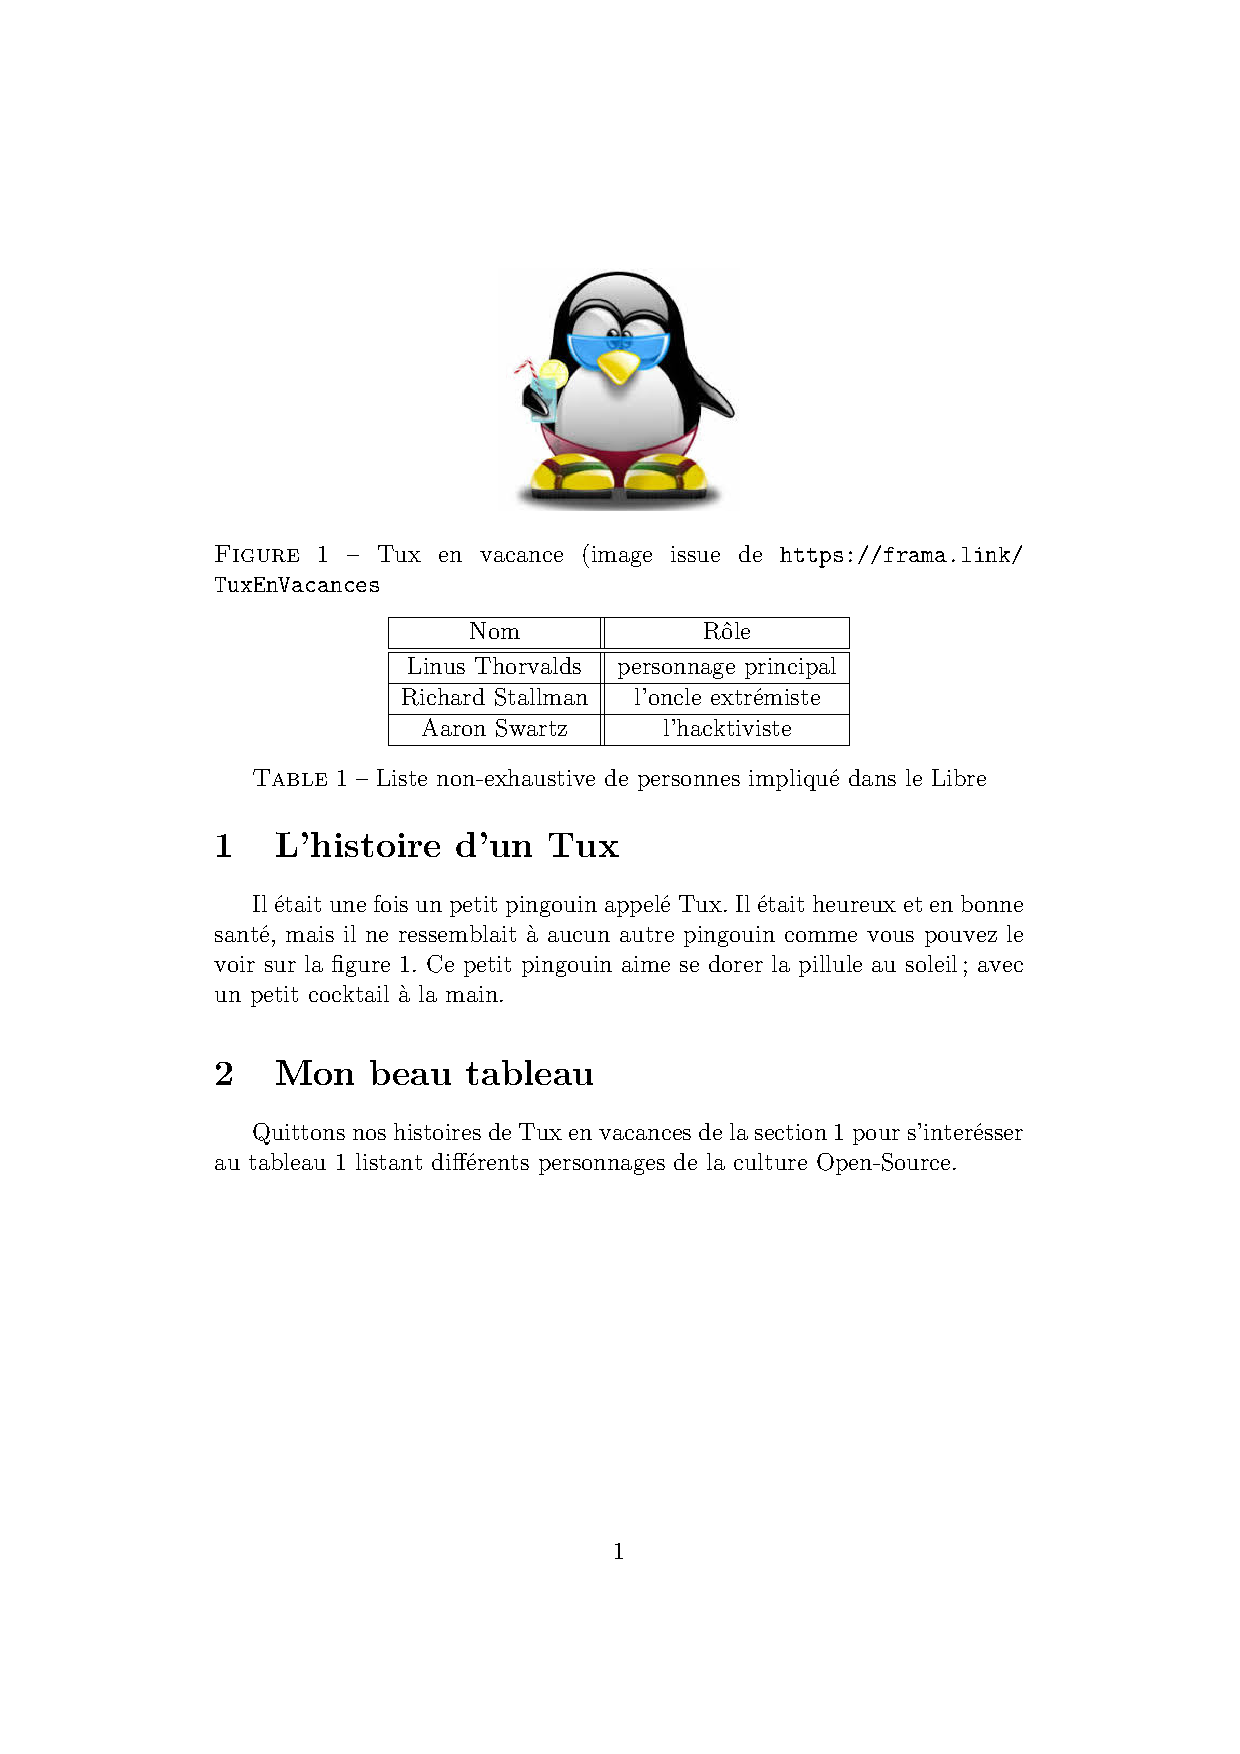
\includegraphics[height=7cm,trim={2cm 8cm 2cm 4cm},clip]{../build_latex/exercices/2/main.pdf}}
  \end{center}
\end{frame}

\begin{frame}[fragile]{Deuxième exercice (solution)}
  \begin{center}
  Lien Overleaf de la solution du deuxième exercice \url{https://www.overleaf.com/read/dmcqrmdjwmdw}
  \end{center}
\end{frame}
